\chapter{Solution proposal}

\textit{The project group went through a discussion for a mobile robotic solution to the problem, the following chapter will describe our thoughts - But bear in mind that this is not an in-depth proposal}

        \vspace{2mm}
        
\begin{wrapfigure}{r}{0.5\textwidth}
    \centering
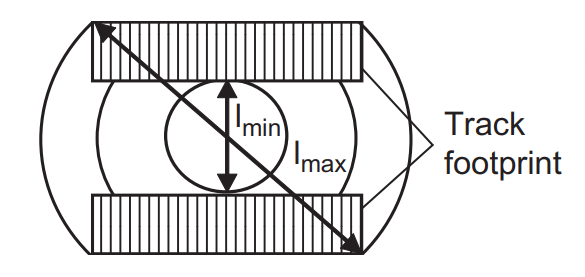
\includegraphics[width=0.45\textwidth]{00 - Images/track_footprint.PNG}
\caption{Illustration of the effective contact point Introduction To Mobile Robot Control \cite{Mobile_robot_control}}
\label{fig:point-of-contact-skid}
\end{wrapfigure}

The solution to the given requirements would be a mobile robot with tracked locomotion or more specifically \textit{"Skid steering"} which is a special integration of differential drive that is usually seen in bulldozers, movers, excavators, and armored vehicles. The main difference from a differential drive wheel-based solution is that the skid-steering has increased maneuverability in uneven terrains due to the higher friction, which is caused by the multiple contact points with the terrain regardless of whether it is rough or even. Figure \ref{fig:point-of-contact-skid} illustrates that the effective point contact is constrained by a rectangular uncertainty area which correlates to the track footprint. The concentric circles illustrate that the vehicle needs a substantial slippage to turn or rotate. \cite{Mobile_robot_control}

\vspace{2mm}
Furthermore the solution proposal should be equipped with a variety of sensors which are explained in the combination with the following mock-up drawings. 

\vspace{4mm}

\begin{figure}[!ht]
  \centering
  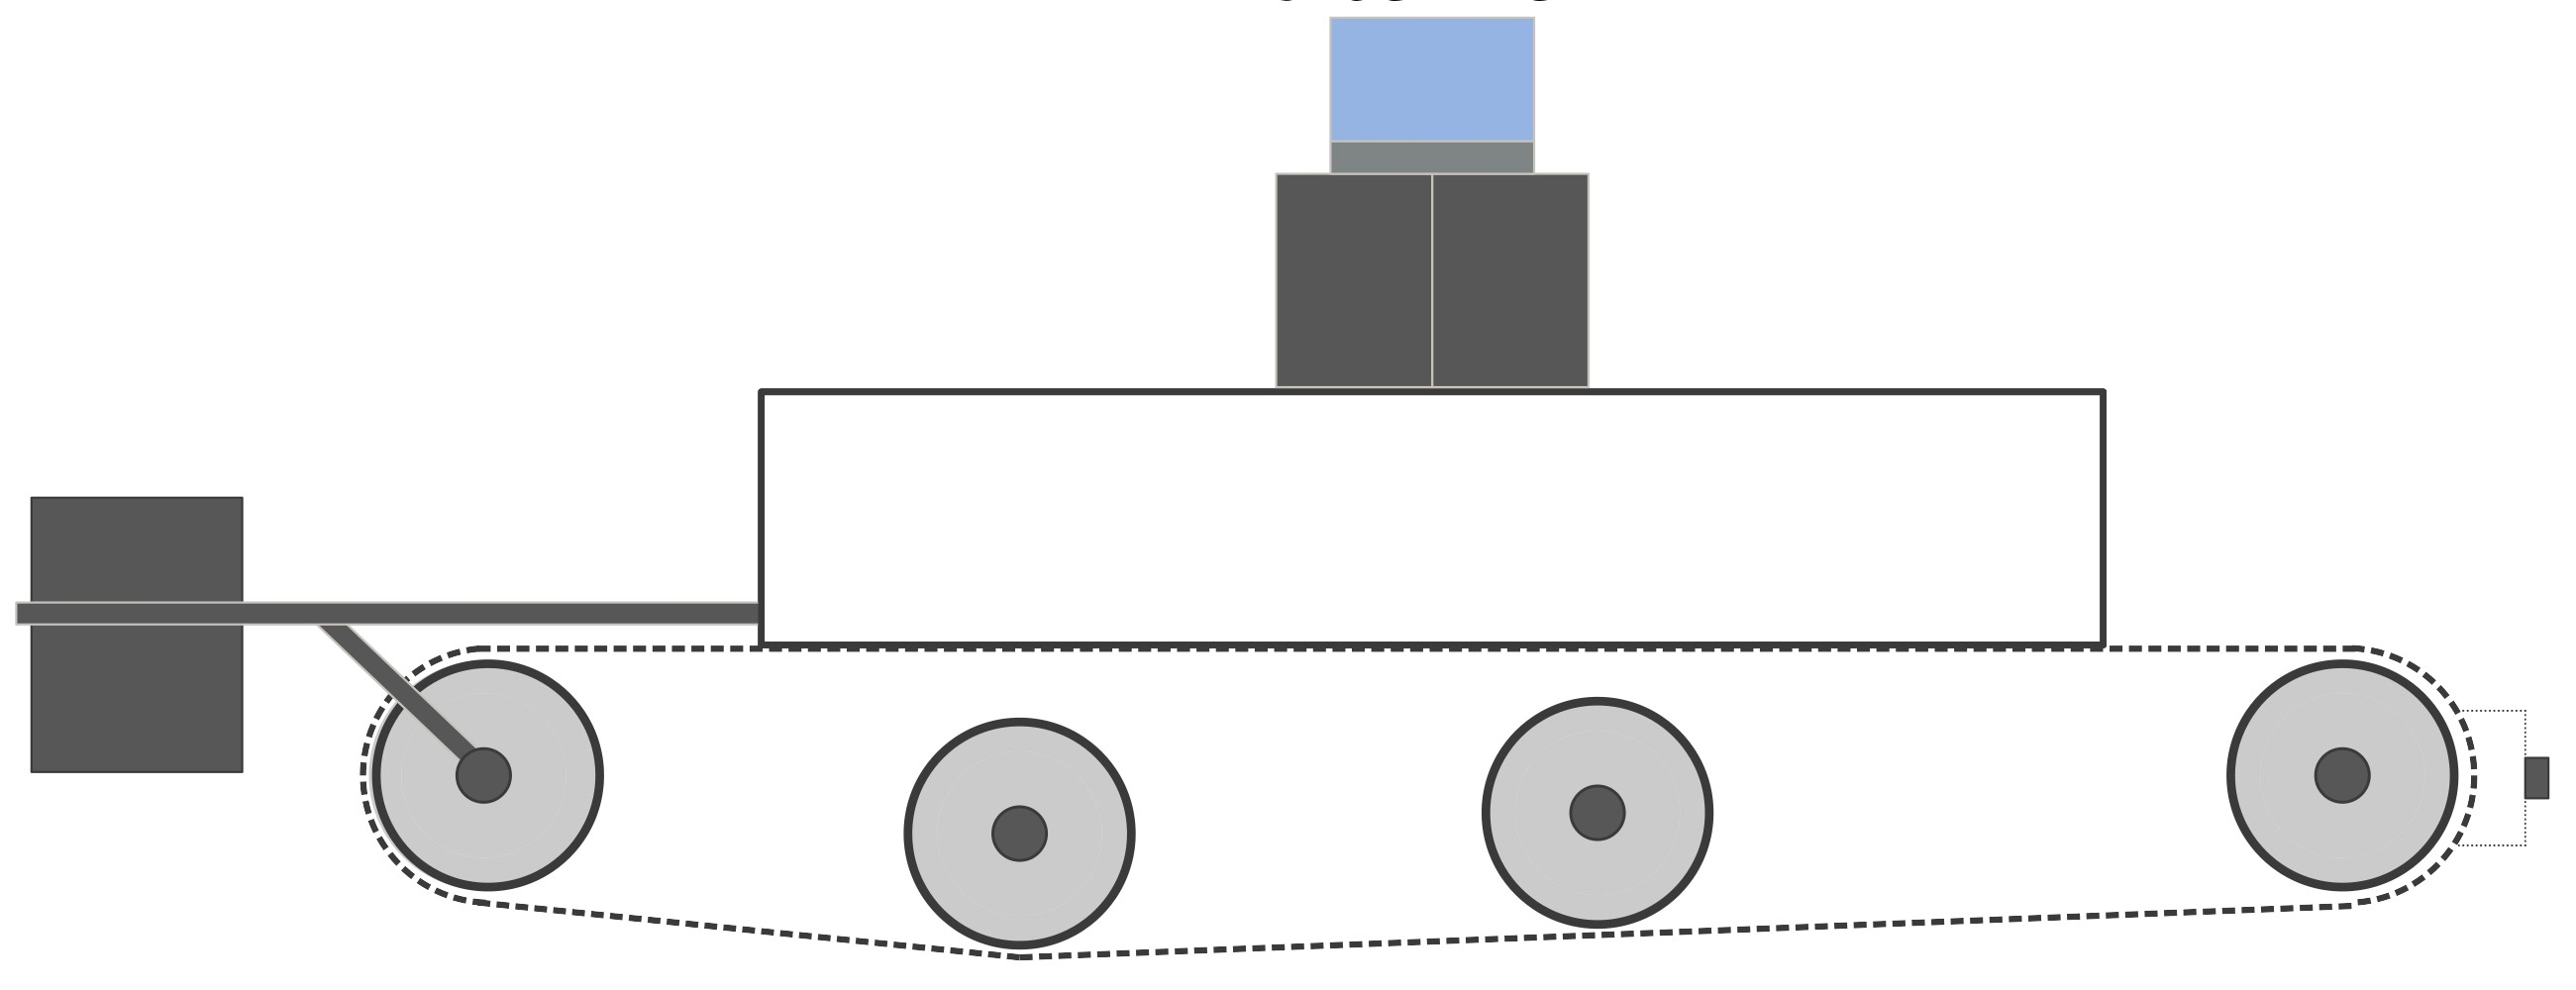
\includegraphics[width=\textwidth]{00 - Images/side_view_sp.jpeg}
  \caption{Side view of the proposed robot}
  \label{fig:side_view_sp,}
\end{figure}

\newpage

\begin{figure}[!ht]
  \centering
  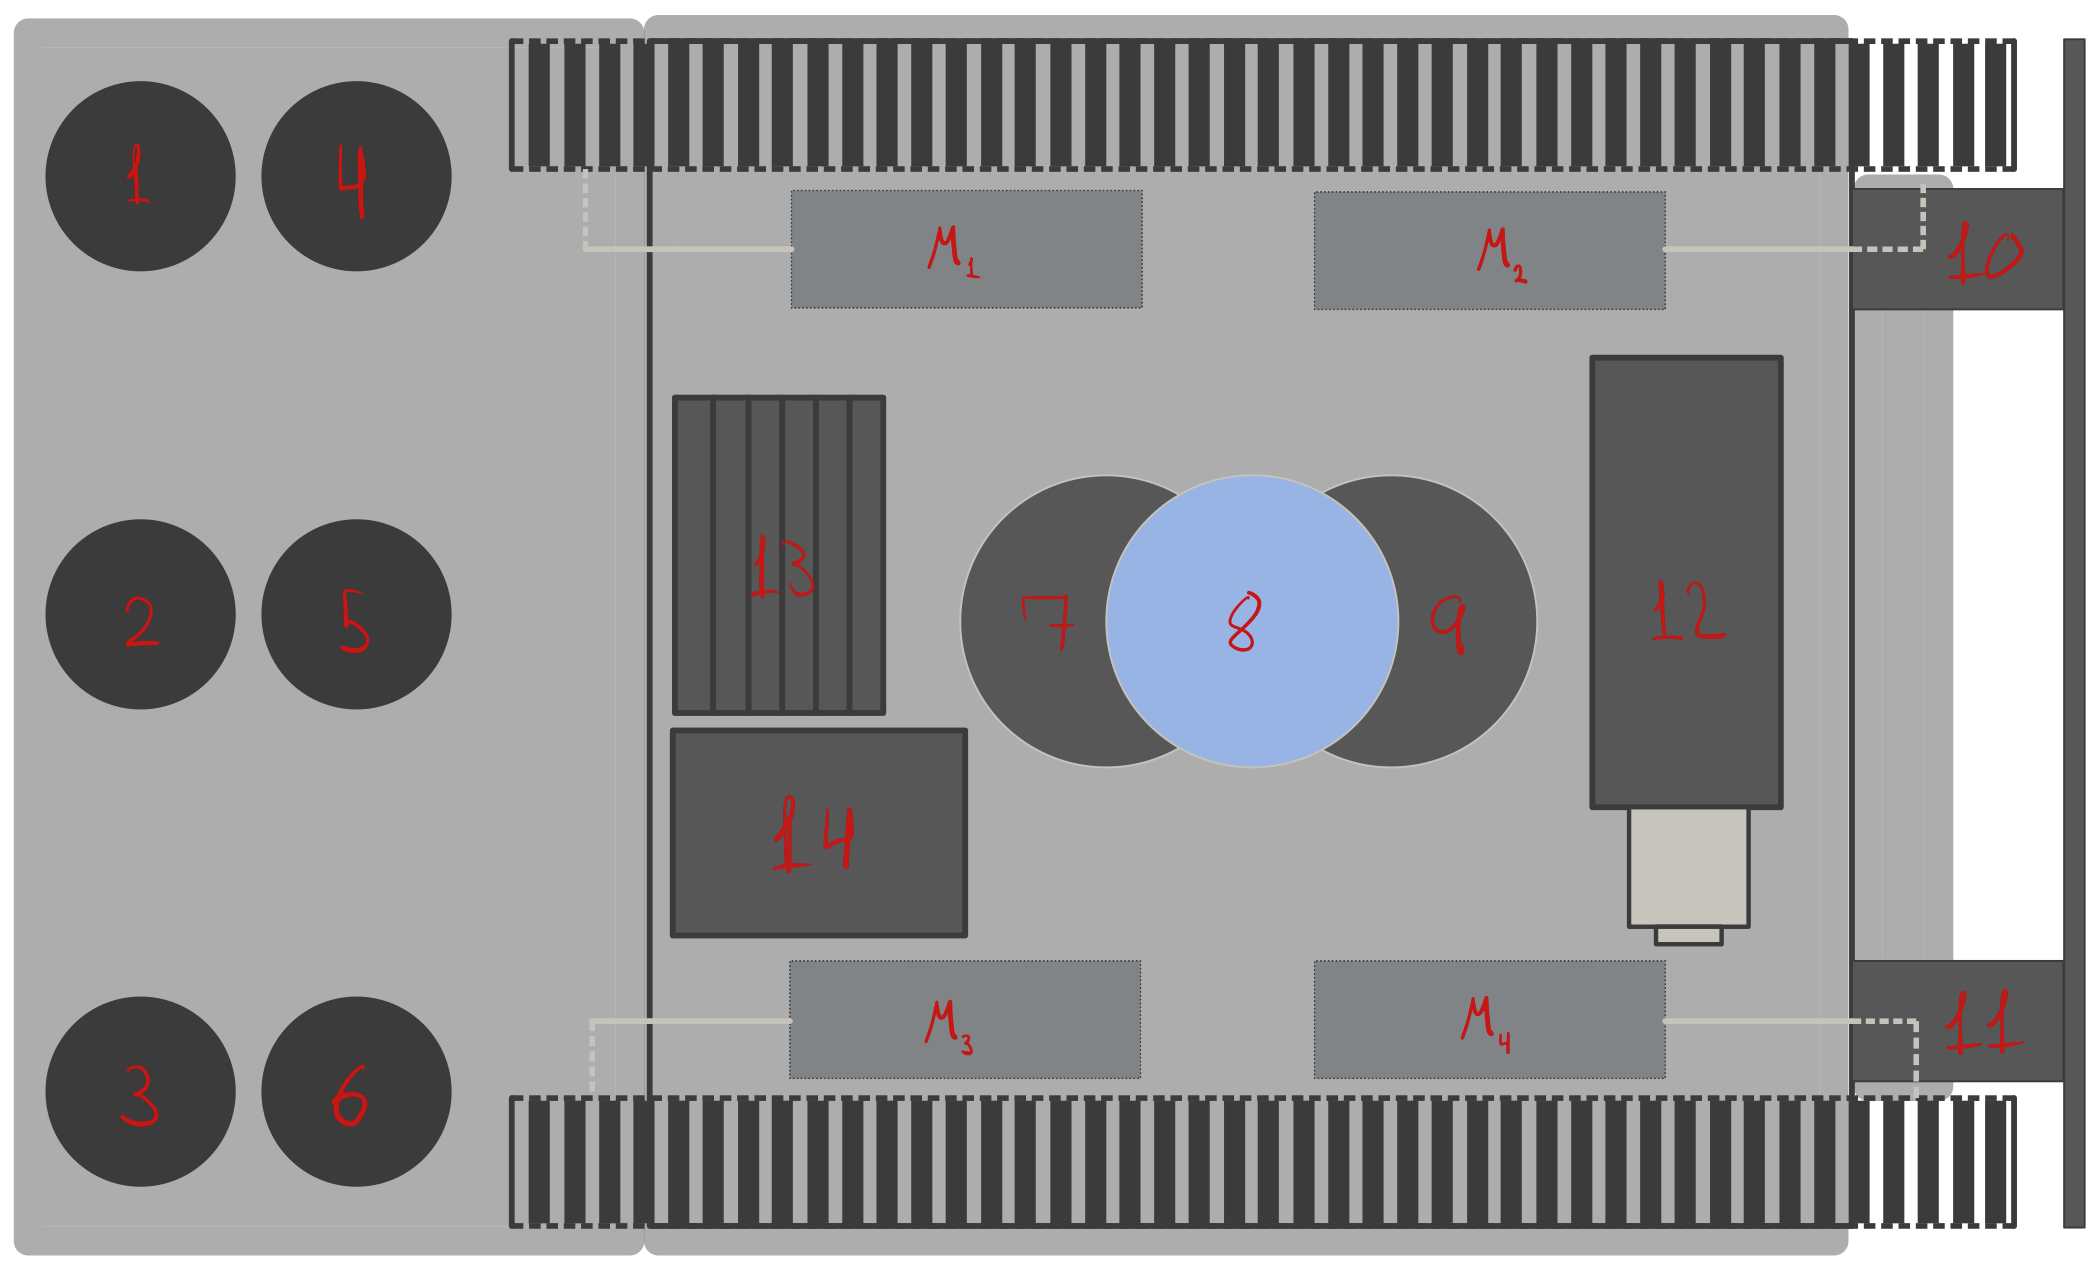
\includegraphics[width=13cm]{tex/00 - Images/top_view_sp2.png}
  \caption{Top view of the proposed robot}
  \label{fig:top_view_sp,}
\end{figure}

  \begin{center}
  \begin{longtable}{| c | L{6cm} | L{3cm} | L{7cm} |}
  \caption{Description for Fig. \ref{fig:top_view_sp,}} \label{tab:top_view} \\
  \hline 
  \multicolumn{1}{|c|}{\textbf{\#}} 
  & \multicolumn{1}{c|}{\textbf{Name}} 
  & \multicolumn{1}{c|}{\textbf{Location}} 
  & \multicolumn{1}{c|}{\textbf{Description}}\\ 
  \hline 
  \endfirsthead
  
  \multicolumn{3}{c}%
  {{\bfseries \tablename\ \thetable{} -- continued from previous page}} \\
  \hline
  \multicolumn{1}{|c|}{\textbf{\#}} 
  & \multicolumn{1}{c|}{\textbf{Name}} 
  & \multicolumn{1}{c|}{\textbf{Location}} 
  & \multicolumn{1}{c|}{\textbf{Description}}\\ 
  \hline 
  \endhead

\hline \hline
\endlastfoot

1 
& Metal detector 
& Right
& For the purpose of detecting metal mines, there are three sensors for the purpose of approximating the mine type.
\\
\hline
2 
& Metal detector 
& Center
& \dittotikz
\\
\hline
3 
& Metal detector 
& Middle
& \dittotikz
\\
\hline
4 
& \gls{gpr} 
& Right
& For the purpose of locating non-metallic mines (Plastic, wood or glass), there are three sensors for the purpose of approximating the mine type.
\\
\hline
5 
& \gls{gpr} 
& Center
& \dittotikz
\\
\hline
6 
& \gls{gpr} 
& Middle
& \dittotikz
\\
\hline
7 
& Pressure chamber (Red paint)
& ND
& Operation defined in Fig. \ref{fig:paint_distro}
\\
\hline
8 
& Sensor tower rack 
& Robot Center
& The tower rack consists of a camera module and a rotating LiDAR sensor for optimized 3D-Mapping and obstacle avoidance.
\\
\hline
9 
& Pressure chamber (Blue paint)
& ND
& Operation defined in Fig. \ref{fig:paint_distro}
\\
\hline
10 
& Rear bumper switch
& Rear-Right
& Bumper switch interconnected with the other rear bumper switch, gives the possibility to see right, left or center surface contact.
\\
\hline
11 
& Rear bumper switch 
& Rear-Left
& \dittotikz
\\
\hline
12
& 12V Compressor
& ND
& For pressurising the paint pressure chambers as shown in Fig.  \ref{fig:paint_distro}
\\
\hline
13
& Battery pack
& ND
& Battery pack for operation.
\\
\hline
14
& Controller units
& ND
& Units for controlling the operation (Raspberry pi, Arduino, etc.)
\\
\hline
ND
& Range sensor
& Bottom
& Downward pointing to ensure that the robot does not drive off a cliff.
\\
\hline
ND
& Gyroscope and accelerometer
& ND
& To make sure the robot wont drive too fast or has turned over.
\\
\hline
ND
& Paint marking nozzle
& ND
& To mark located mines: Red or blue paint
\\
\hline
$M_1$
& Servo motor 
& Right-Front
& Each servo motor serves the purpose of rotating or stopping the track, which corresponds to a differential drive tracked solution.
\\
\hline
$M_2$
& Servo motor 
& Right-Rear
& \dittotikz
\\
\hline
$M_3$ 
& Servo motor 
& Right-Left
& \dittotikz
\\
\hline
$M_4$
& Servo motor 
& Left-Rear
& \dittotikz
\\
\hline
\end{longtable}
\end{center}

\begin{figure}[!ht]
    \centering
    \begin{minipage}{0.5\textwidth}
        \centering
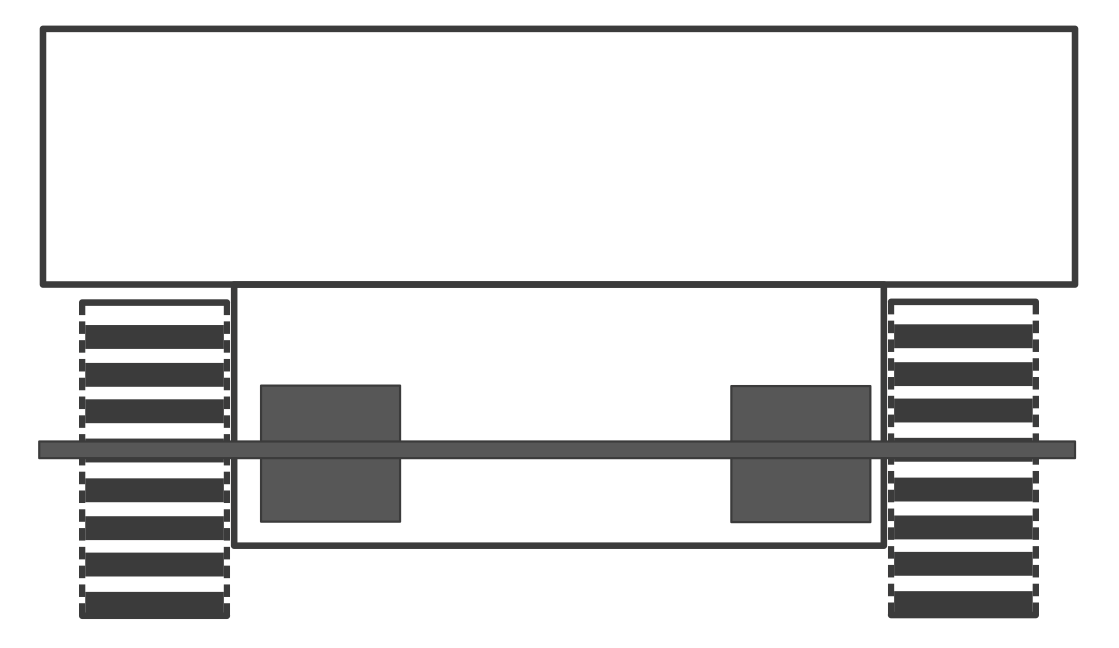
\includegraphics[width=0.9\textwidth]{00 - Images/rear_view_sp.png}
\caption{Rear view of the proposed robot}
    \end{minipage}\hfill
    \begin{minipage}{0.5\textwidth}
        \centering
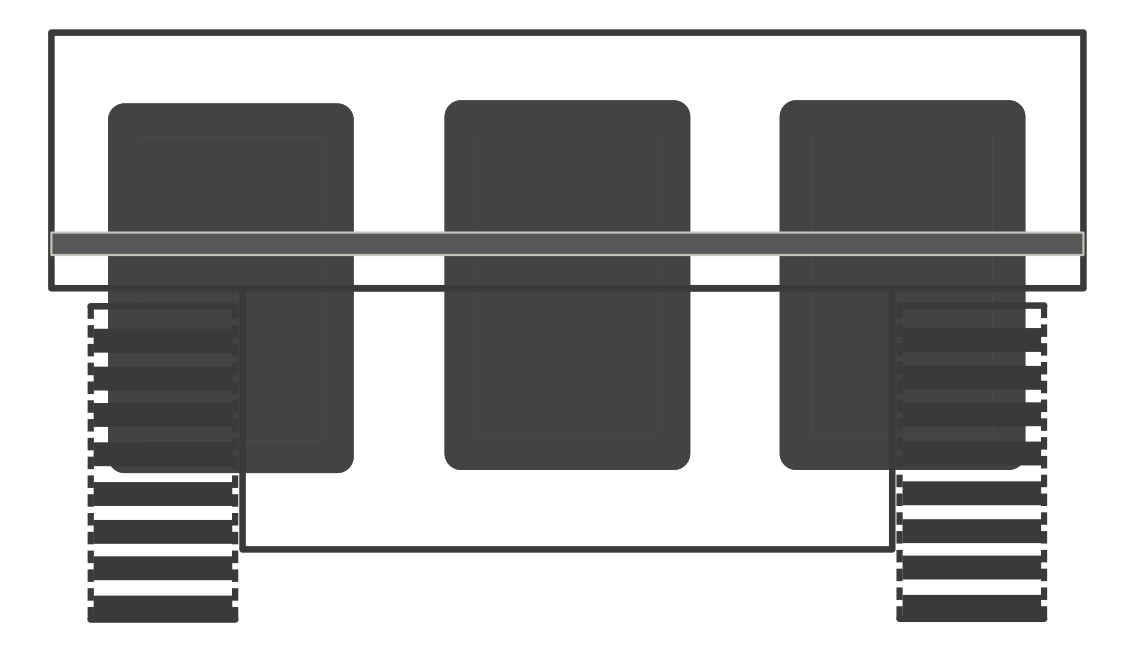
\includegraphics[width=0.9\textwidth]{00 - Images/front_view_sp.jpeg}
\caption{Front view of the proposed robot}
    \end{minipage}
\end{figure}

\newpage

\section*{Paint distribution system}

\begin{figure}[!ht]
  \centering
  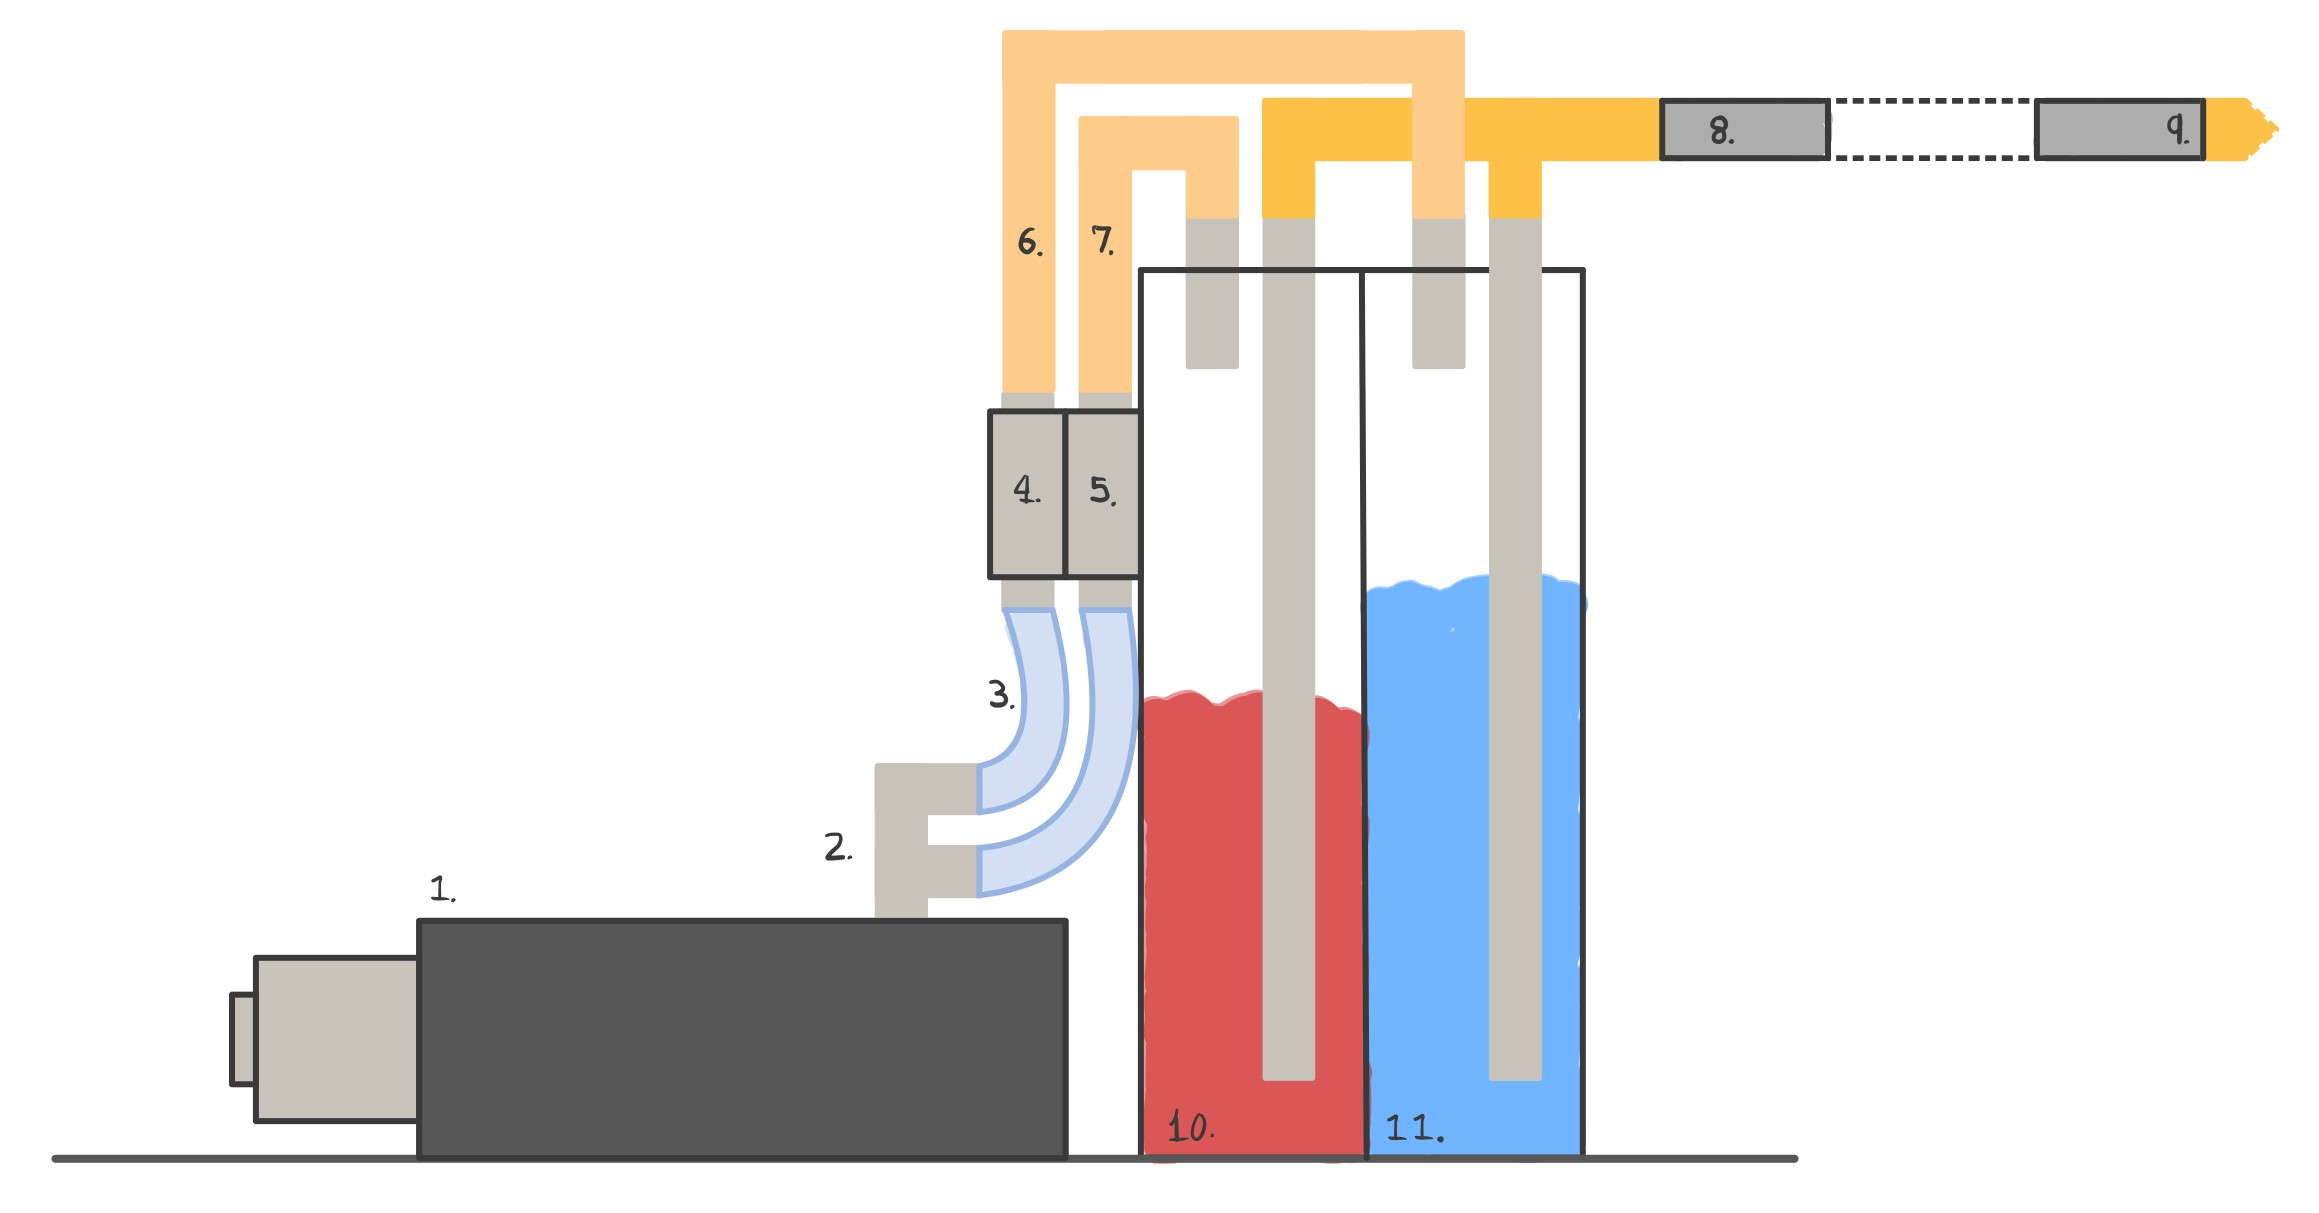
\includegraphics[width=\textwidth]{00 - Images/paint_disto_sp.jpeg}
  \caption{Side and X-Ray view of the paint distrobtion marking solution}
  \label{fig:paint_distro}
\end{figure}

The paint distribution unit is used by the robot to mark mines in a color depending on the specified mine type. It functions in the following way: \textbf{The compressor (1)} has a pressure chamber which holds a steady PSI through the \textbf{pressure splitter (2)}, this splitter is connected with \textbf{HP\footnote{HP stands for "High Pressure"} tubing (3)} to both \textbf{magnetic valve 1 (4)} and \textbf{magnetic valve 2 (5)} which acts a stopping valve for the pressure. 

\vspace{2mm}

When a signal is sent to one of the magnetic valves, the pressure is transmitted through their respective \textbf{HP copper tubing (6, 7)}, which is connected to their own respective \textbf{HP Chambers (10, 11)}.

\vspace{2mm}

Inside these chambers, the pressure is added at the top which forces the paint through the tubes extended into the paint. From this point, the paint travels in a pressurized state from the \textbf{nozzle extension (8)} to the \textbf{end of nozzle extension (8)} where it is sprayed upon the surface that the nozzle is pointing at.